\subsection{Software Development}
Any aircraft participating in the UAV Challenge must be autonomous, only interacting with a human to be armed or disarmed at the beginning and end of the mission. A framework for autonomous flight was developed in Python for the Raspberry Pi, based on the following considerations:
\begin{itemize}
	\item Extendibility: Software is designed so that future teams can easily add functionality to the autonomous systems
	\item Concurrency: Software launches several parallel processes, enabling real-time interaction between the many subsystems of the aircraft and software
	\item Low-Latency: All processes must little to no delays in communication, allowing for real-time operation 
\end{itemize}

Figure \ref{fig:softwarearchitecture} shows the software architecture for the autonomous flight and intelligence systems implemented on the Raspberry Pi, consisting of a number of parallel processes, two objects to monitor the state of the aircraft, and objects to facilitate communication between the processes. Each process shown in Figure \ref{fig:softwarearchitecture} performs a specific function:
\begin{itemize}
	\item \textbf{Autopilot:} Acts as an interface to pass flight commands from the UAV software to the PixHawk, and respond to sensor data
	\item \textbf{Flight:} Generates the desired flight path for the aircraft, sends flight commands to the Autopilot process
	\item \textbf{UAVStateUpdater:} Monitors and updates the state of the aircraft by interfacing with sensors, including GPS, accelerometer, etc; manages the UAVState object that stores sensor data
	\item \textbf{WorldStateUpdater:} Monitors and updates the state of the world by interfacing with sensors, including camera, LiDAR and ultrasonic; manages the WorldState object that stores sensor data
	\item \textbf{BaseCommunications:} Provides a real-time data link between the aircraft and the ground station
	\item \textbf{Logging:} Retrieves data from other modules and generates flight logs for reviewing mission performance
\end{itemize}

\begin{figure}[!ht]
	\centering
	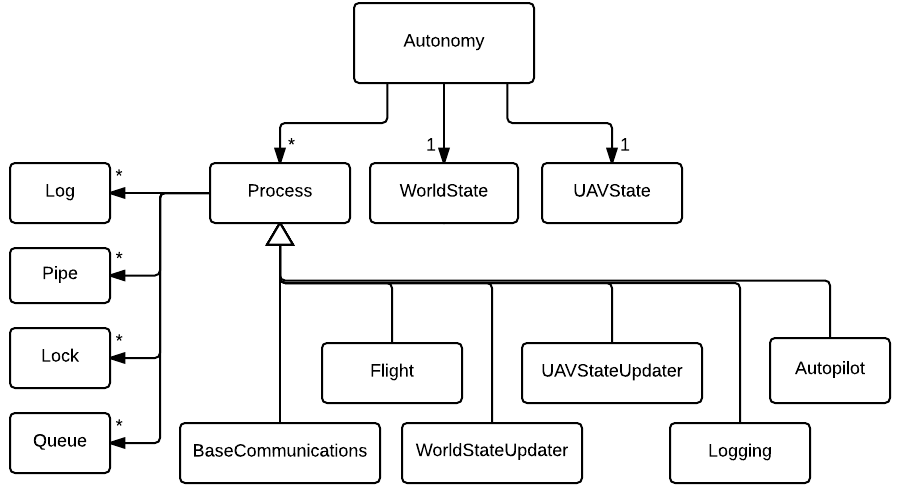
\includegraphics[width=340pt]{\IMAGEPATH /Diagrams/software}
	\caption{High level software architecture}
	\label{fig:softwarearchitecture}
\end{figure}

Figure \ref{fig:softwareinteraction} shows the communication paths between the various processes. As a result of the multiprocessing framework, communication between modules is not as simple as passing variables through functions. Instead, whenever two or more processes communicate with each other, a dedicated ``link'' needs to be created between them. Pipes (blue in Figure \ref{fig:softwareinteraction}) allow for bidirectional communication between processes, such as between the Flight and Autopilot. Queues (green in Figure \ref{fig:softwareinteraction}) only allow unidirectional communication, such as between all processes and the Log process.\\

One of the biggest dangers in parallel processing communication is data corruption or loss; one process attempts to read data from a link while another is modifying or writing to it. To prevent this, each process that connects with either a pipe or queue is provided with read and write ``locks''. When activated, the lock will prevent other processes from reading from, or writing to, the communication link before the current process is finished with it.

\begin{figure}[H]
	\centering
	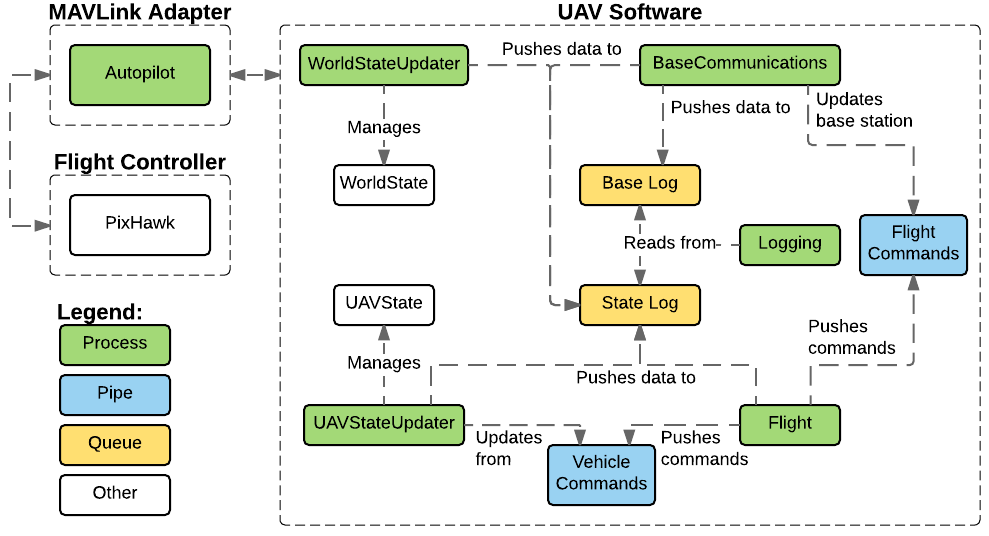
\includegraphics[width=380pt]{\IMAGEPATH /Diagrams/interaction}
	\caption{Interaction between software modules}
	\label{fig:softwareinteraction}
\end{figure}

\subsection{Testing}
Before being implemented on the prototype aircraft, the autonomous flight modules were first tested in a simulated aircraft using ArduPilot's Software in the Loop capabilities\cite{ref:sitl}. Figure \ref{fig:sitl} shows a screenshot of the mission simulation, where the virtual aircraft was successfully tested with the software discussed above, executing a simple mission consisting of a series of \textbf{M1} commands; takeoff to 10m, forward flight of 10m, and landing.

\begin{figure}[H]
	\centering
	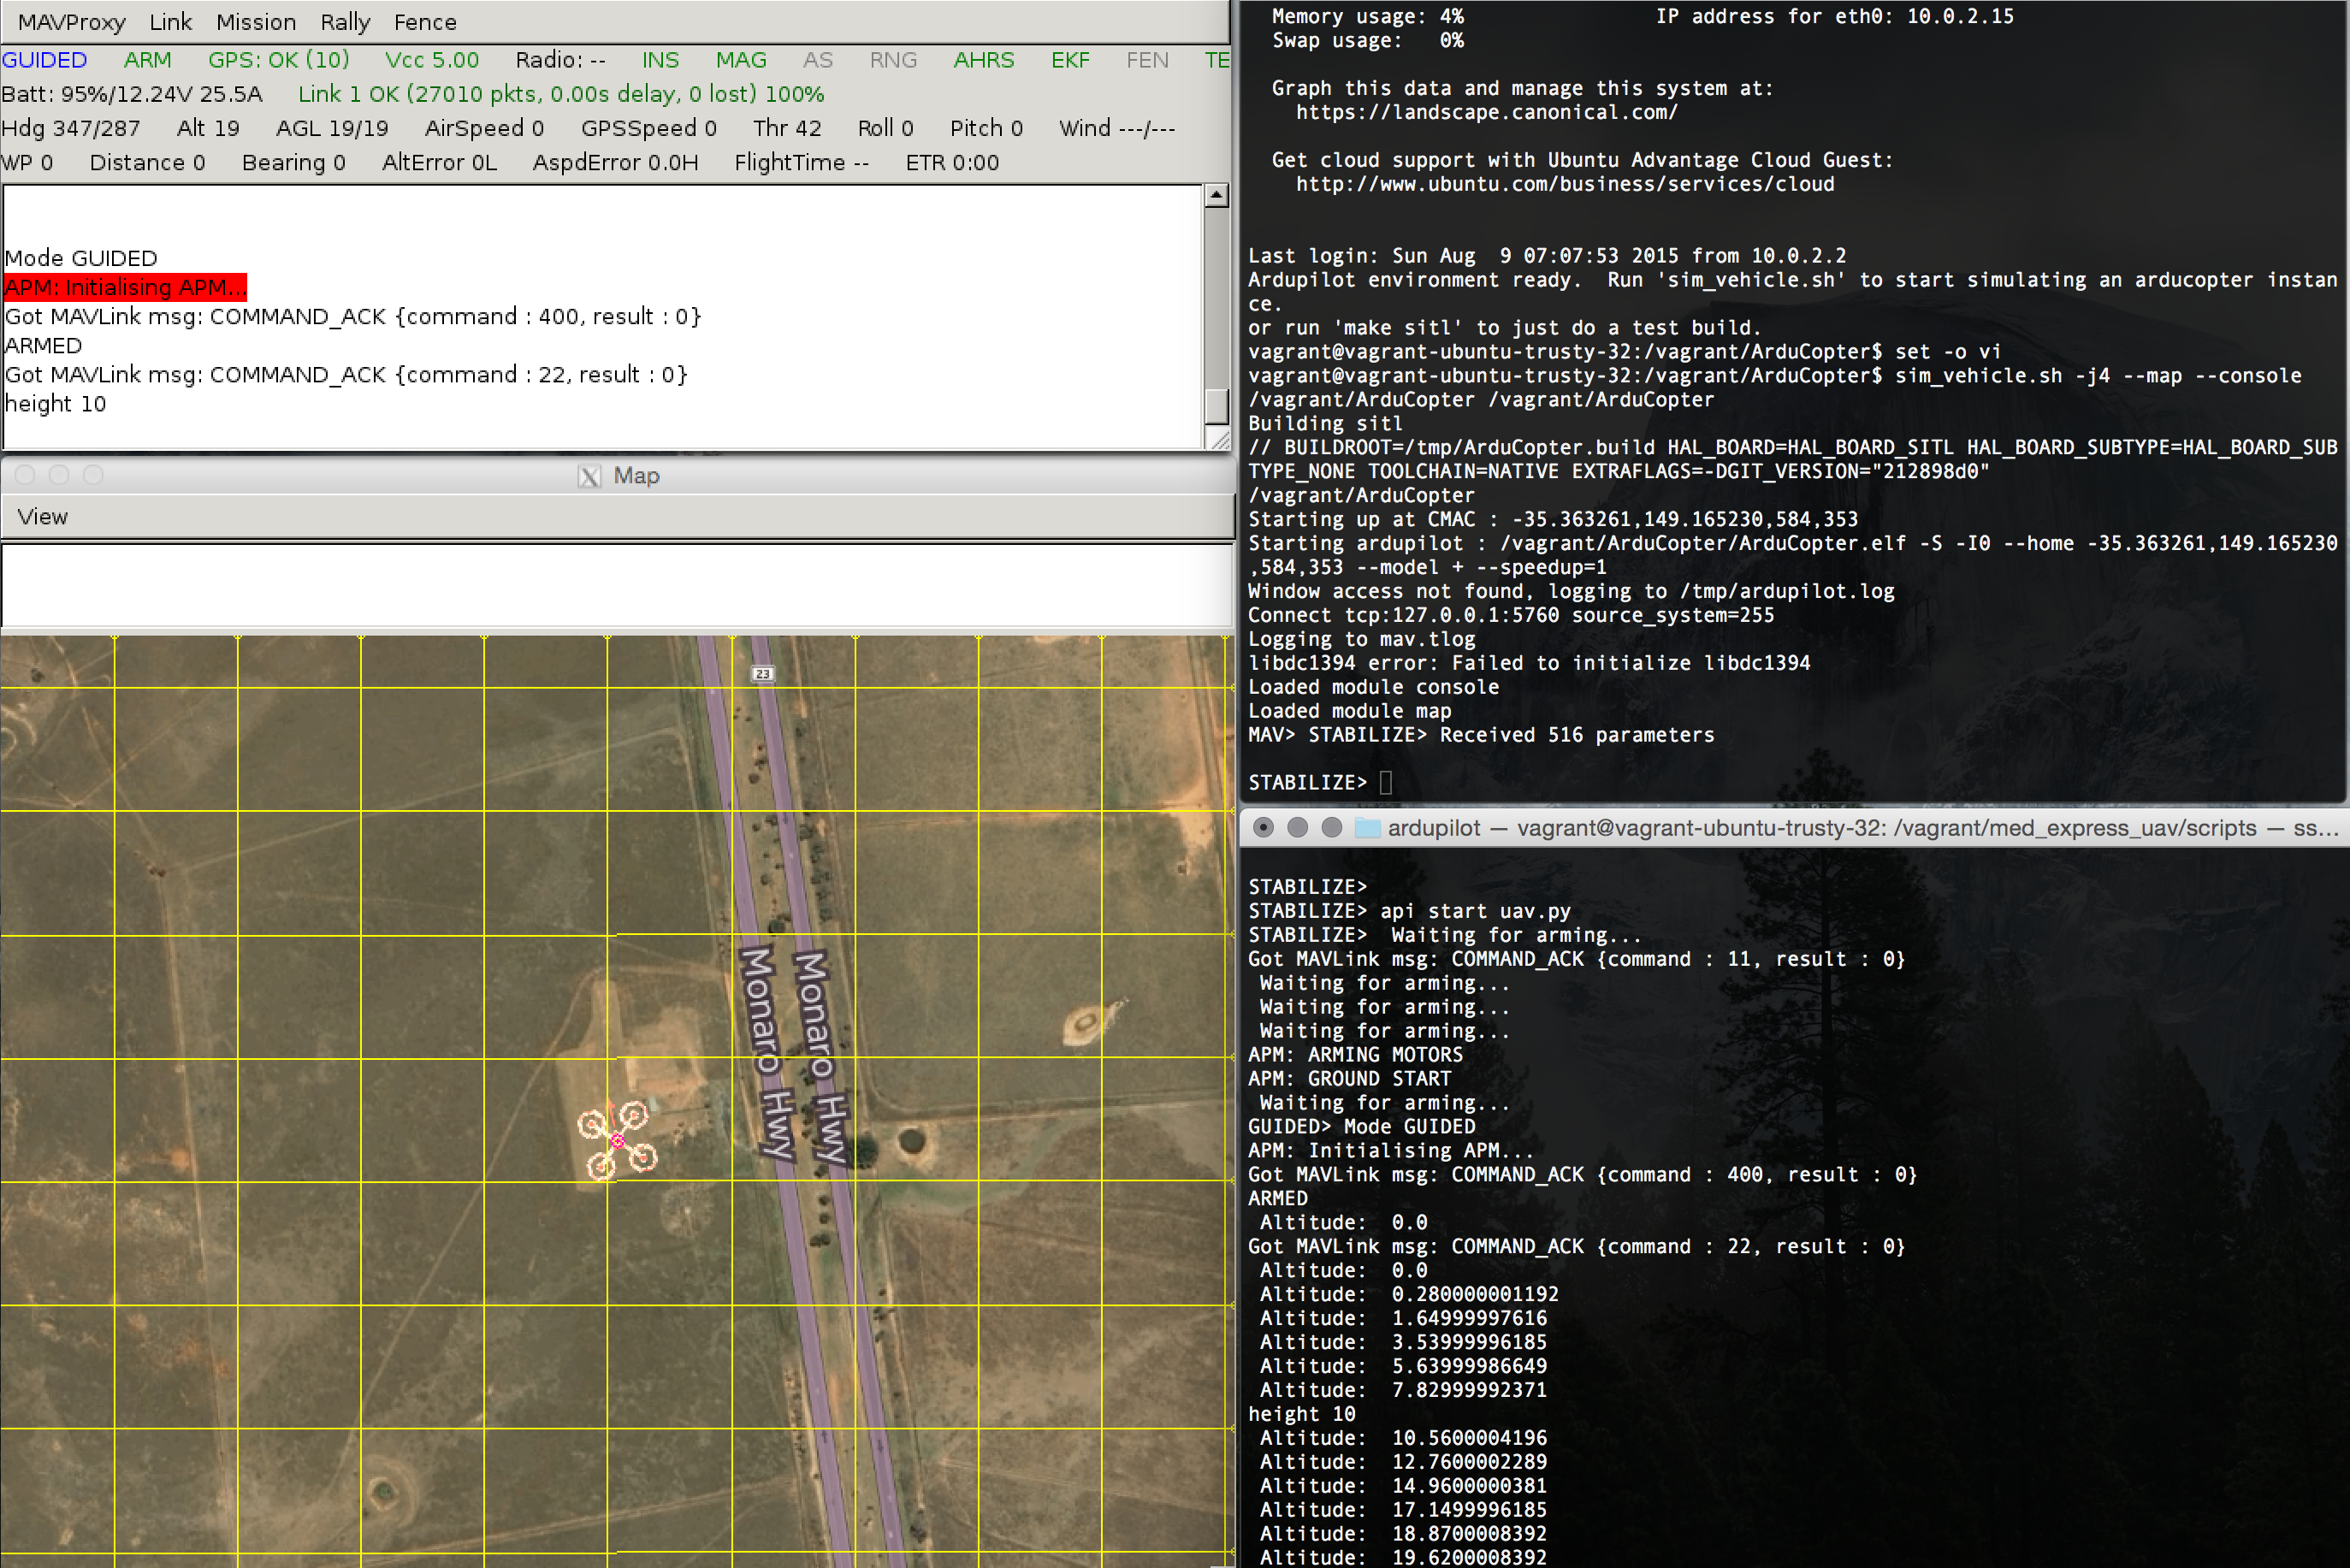
\includegraphics[width=400pt]{\IMAGEPATH /Diagrams/sitl}
	\caption{Software in the Loop testing}
	\label{fig:sitl}
\end{figure}